% !TEX program = xelatex
\documentclass[aspectratio=169, xcolor=dvipsnames]{beamer}
\usetheme{metropolis}

% metropolis theme was built with Fira font in mind...
\setsansfont[
  Path = ../.fonts/,
  Extension = .ttf,
  UprightFont = *-Regular,
  ItalicFont = *-Italic,
  BoldFont = *-Bold,
  BoldItalicFont = *-BoldItalic
]{FiraSans}

\setmonofont[
  Path = ../.fonts/,
  Extension = .ttf,
  UprightFont = *-Regular,
  BoldFont = *-Bold
]{FiraMono}

\graphicspath{{../figures/}}

\usepackage{listings}
\lstset{
  basicstyle=\ttfamily, % use Fira font
  columns=fullflexible
}
\usepackage{tikz}
\usetikzlibrary{matrix}
\usetikzlibrary{positioning}
\usepackage[style=authoryear, backend=biber]{biblatex}
\addbibresource{bibliography.bib}

\title{Cache Optimization: Better for Big Data?}
\subtitle{Cache-Oblivious Algorithms for High-Latency Memory Transfers} % some tagline, can be changed if we want
\date{\today}
\author{Logan Decock \and Juan Rempel}
\institute{University of Manitoba\\Advanced Data Structures and Algorithms}

\begin{document}

\maketitle

\section{Introducing the \\Cache-Oblivious Model}

% 15 seconds
\begin{frame}{Why?}
    \begin{columns}[T]
        \begin{column}{0.48\textwidth}
            Memory: slow
            \begin{figure}
                \centering
                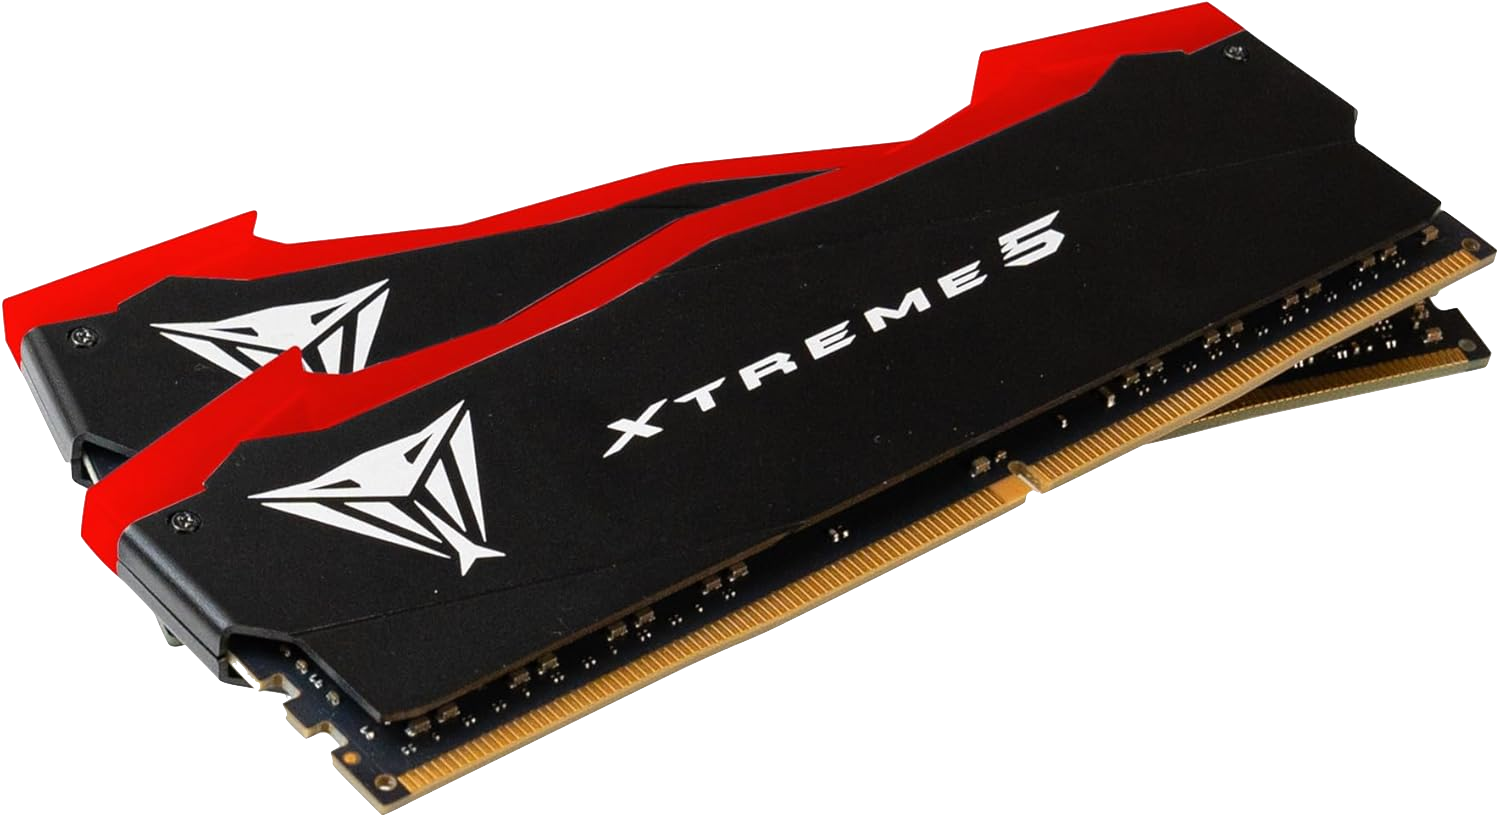
\includegraphics[height=0.25\textwidth]{image1.png}
                \caption{Viper5 DDR5 6000MT/s CL30}
            \end{figure}
            \vspace{-15pt}
            \footnotesize
            \begin{align*}
                \text{Latency (ns)} 
                &= \frac{2000 \cdot \text{CAS Latency}}{\text{RAM speed in MT/s}} = \frac{2000 \cdot 30}{6000} \\
                &= 10 \text{ ns}
            \end{align*}
            
        \end{column}

        \begin{column}{0.48\textwidth}
            CPU: fast
            \begin{figure}
                \centering
                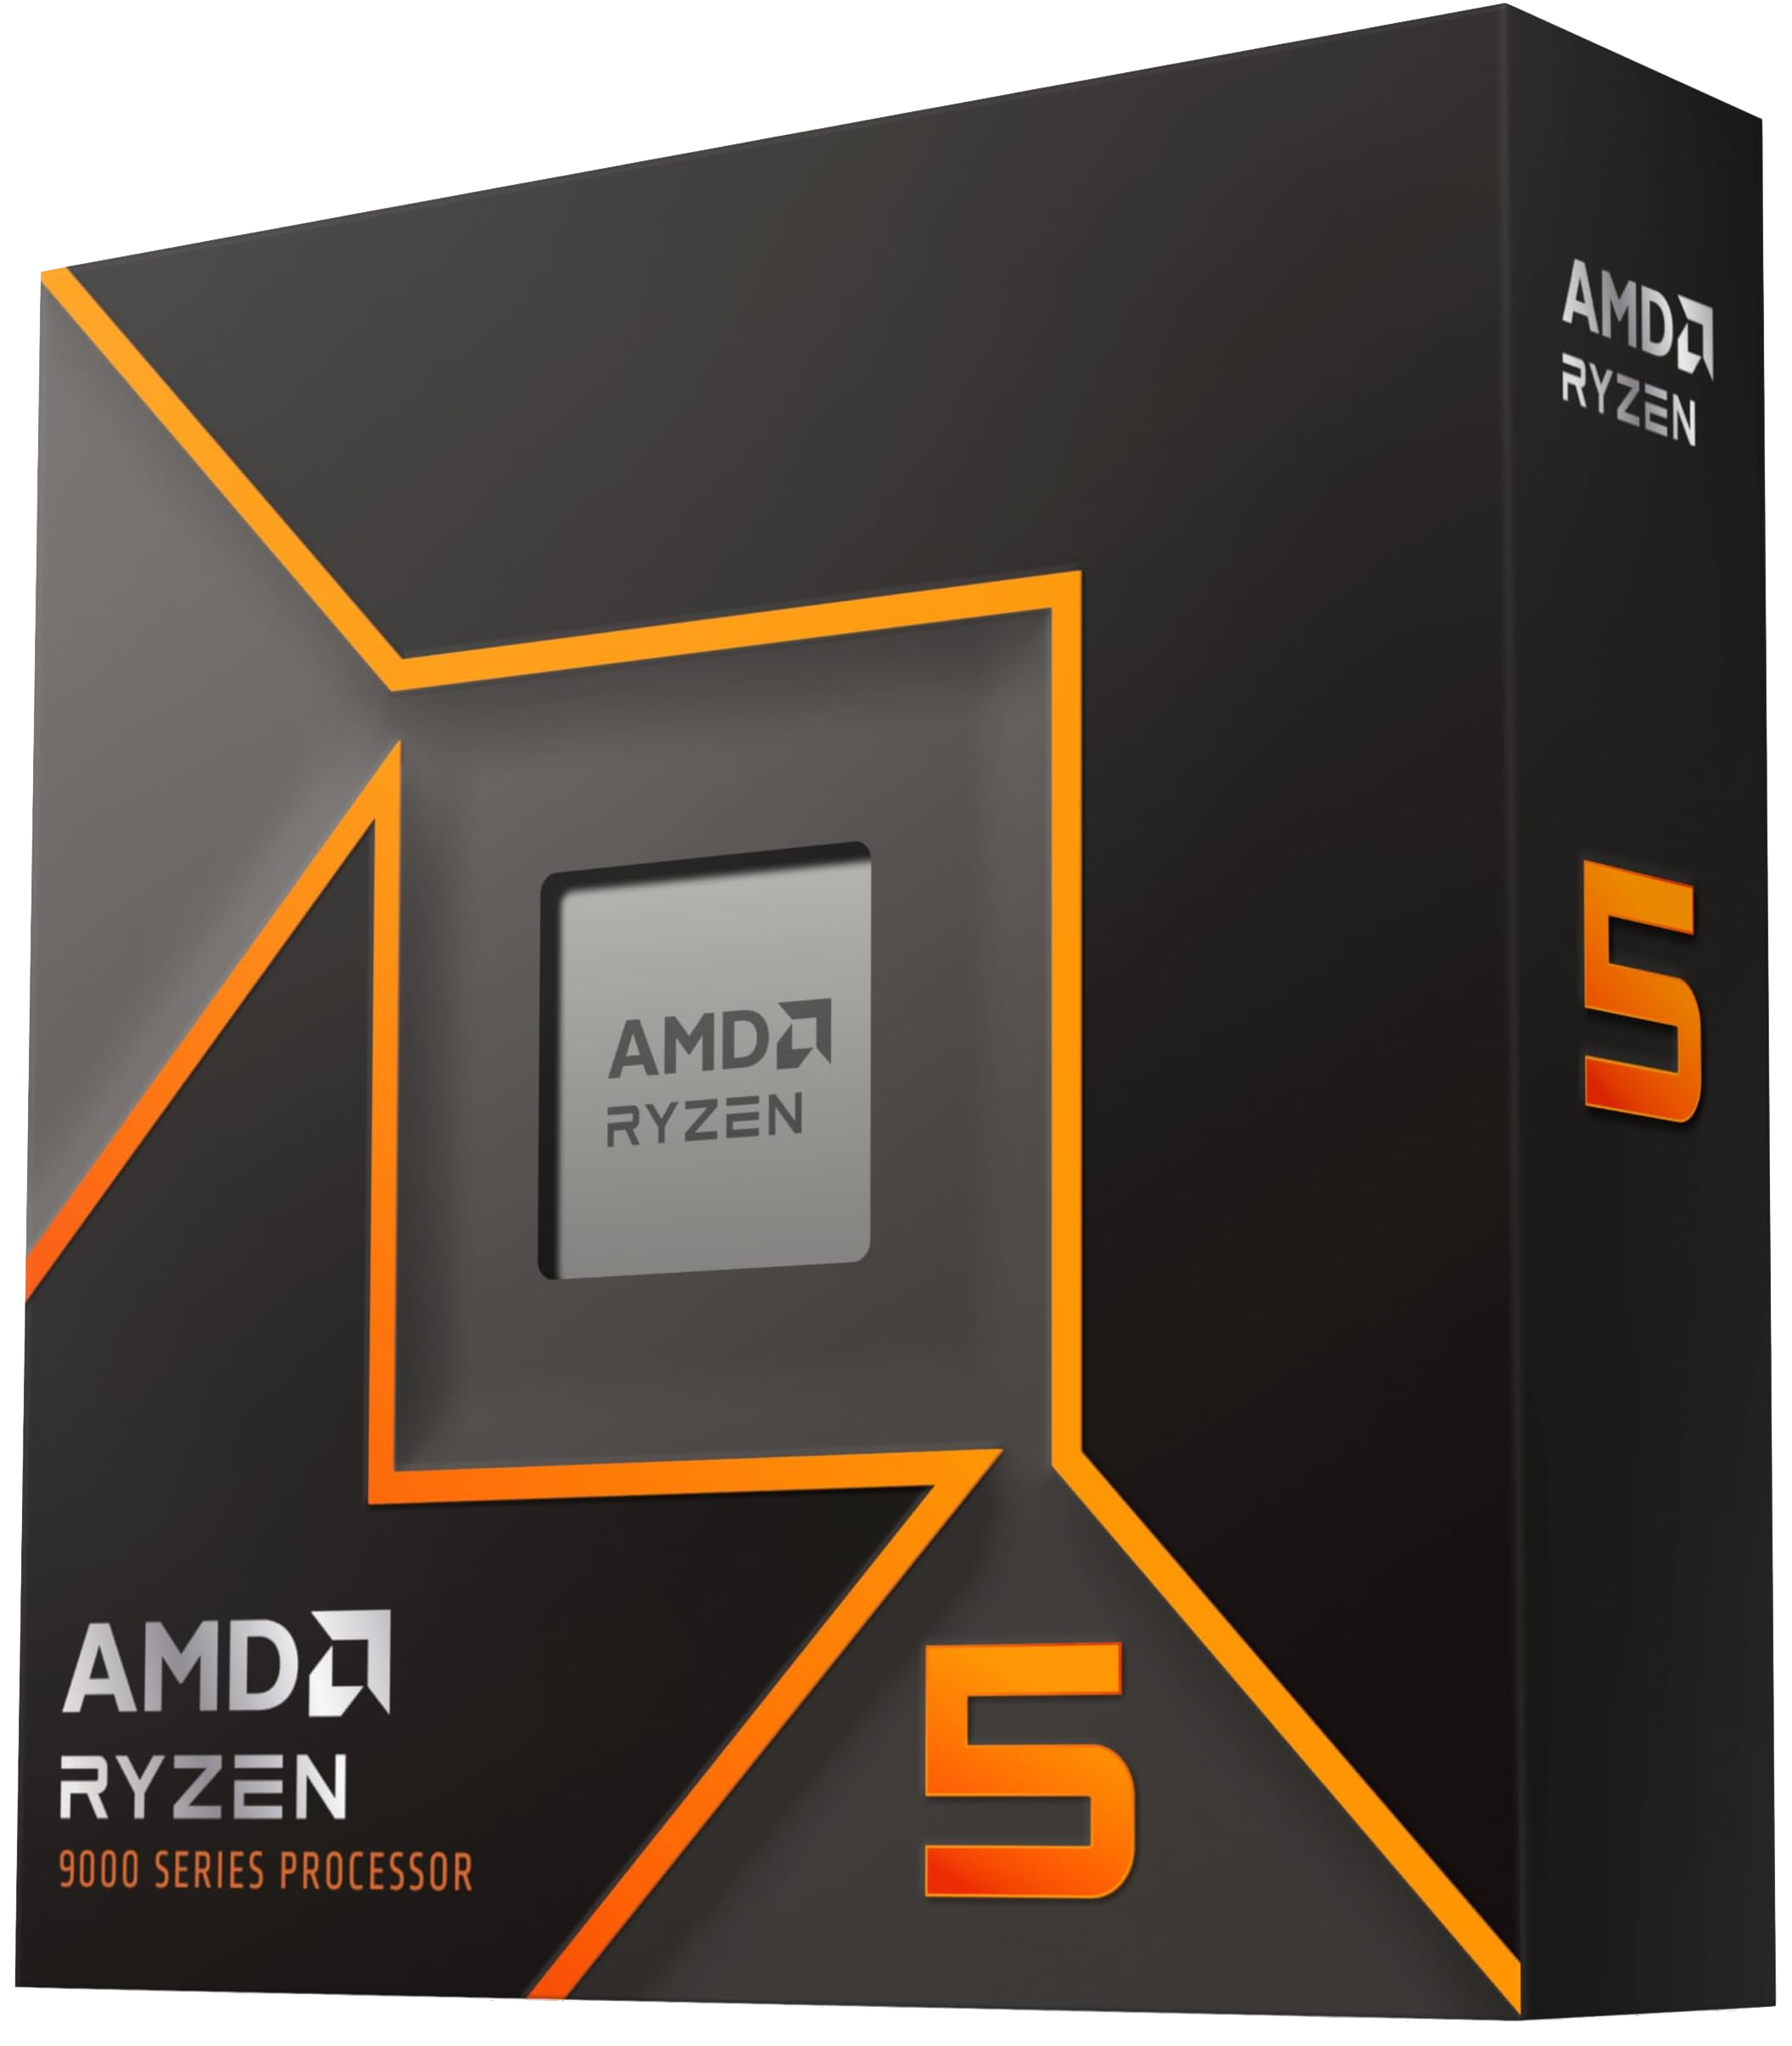
\includegraphics[height=0.25\textwidth]{image2.png}
                \caption{AMD Ryzen 5 9600X 5.4GHz}
            \end{figure}
            \quad $ 5.4 \text{GHz} = 5.4 \text{ clock cycles per ns} $
        \end{column}
    \end{columns}

    $10 \text{ ns delay in memory fetch } \implies \text{ stalled for $54$ clock cycles} $

    \textit{Can we optimize algorithms for this? Yes. Yes we can.}

    \bigskip
    \vfill
    \tiny \textcolor{gray}{Sources - Images: amazon.ca - Math: kingston.com}
\end{frame}


% 15 seconds
\begin{frame}{Assumptions}
    \textbf{Word RAM Model:}
    \begin{itemize}
        \item memory transfers are free
        \item instructions cost
        \begin{itemize}
            \item optimize the \# of instructions $\implies$ \textit{no longer care about this}
        \end{itemize}
    \end{itemize}
    \textbf{Cache-Oblivious Model:}
    \begin{itemize}
        \item instructions are free
        \item memory transfers cost
        \begin{itemize}
            \item optimize the \# of memory transfers $\implies$ \textit{want this}
        \end{itemize}
    \end{itemize}
\end{frame}

\begin{frame}[fragile]{Refresher: Cache, Words and Blocks}

    \centering
    \begin{tikzpicture}
    % cache
    \matrix (cache) [matrix of nodes, 
                nodes={inner sep=0pt, minimum width=0.1cm, minimum height=0.4cm, anchor=center}, 
                nodes in empty cells,
                column sep=0pt, 
                row sep=0pt,
                row 6/.style={nodes={fill=mLightBrown!40}}] 
    {
         &&&&&&&&&&&&&&&&&&&&&&&&&&&&&& \\ % line 1
         &&&&&&&&&&&&&&&&&&&&&&&&&&&&&&  \\ % line 2
         &&&&&&&&&&&&&&&&&&&&&&&&&&&&&&  \\ % line 3
         &&&&&&&&&&&&&&&&&&&&&&&&&&&&&&  \\ % line 4
         &&&&&&&&&&&&&&&&&&&&&&&&&&&&&&  \\ % line 5
         &&&&&&&&&&&&&&&&&&&&&&&&&&&&&&  \\ % line 6
         &&&&&&&&&&&&&&&&&&&&&&&&&&&&&&  \\ % line 7
         &&&&&&&&&&&&&&&&&&&&&&&&&&&&&&  \\ % line 8
         &&&&&&&&&&&&&&&&&&&&&&&&&&&&&&  \\ % line 9
         &&&&&&&&&&&&&&&&&&&&&&&&&&&&&&  \\ % line 10
         &&&&&&&&&&&&&&&&&&&&&&&&&&&&&&  \\ % line 11
        %  &&&&&&&&&&&&&&&&&&&&&&&&&&&&&&  \\ % line 12
        %  &&&&&&&&&&&&&&&&&&&&&&&&&&&&&&  \\ % line 13
        %  &&&&&&&&&&&&&&&&&&&&&&&&&&&&&&  \\ % line 14
        %  &&&&&&&&&&&&&&&&&&&&&&&&&&&&&&  \\ % line 15
        %  &&&&&&&&&&&&&&&&&&&&&&&&&&&&&&  \\ % line 16
    };

    % rectangle lines
    \draw (cache-1-1.north west) -- (cache-1-31.north east);
    \draw (cache-1-31.north east) -- (cache-11-31.south east);
    \draw (cache-11-31.south east) -- (cache-11-1.south west);
    \draw (cache-11-1.south west) -- (cache-1-1.north west);

    % row lines
    \foreach \i in {1, ..., 11} {
        \draw (cache-\i-1.south west) -- (cache-\i-31.south east);
    }

    % label
    \node (cachelabel) at ([yshift=0.1cm]cache.north) {\textbf{Cache}};

    % width
    \draw[<->, thick] ([yshift=-0.3cm]cache-11-1.south west) -- ([yshift=-0.3cm]cache-11-31.south east) node[midway, below] {$1$ block $ = B$ words};

    % memory
    \matrix (memory) [right=3cm of cache,
                matrix of nodes, 
                nodes={inner sep=0pt, minimum width=0.1cm, minimum height=0.4cm, anchor=center}, 
                nodes in empty cells,
                column sep=0pt, 
                row sep=0pt,
                row 3/.style={nodes={fill=mDarkBrown!40}}] 
    {
         &&&&&&&&&&&&&&&&&&&&&&&&&&&&&& \\ % line 1
         &&&&&&&&&&&&&&&&&&&&&&&&&&&&&&  \\ % line 2
         &&&&&&&&&&&&&&&&&&&&&&&&&|[fill=mLightGreen!30]|&&&&&  \\ % line 3
         &&&&&&&&&&&&&&&&&&&&&&&&&&&&&&  \\ % line 4
         &&&&&&&&&&&&&&&&&&&&&&&&&&&&&&  \\ % line 5
         &&&&&&&&&&&&&&&&&&&&&&&&&&&&&&  \\ % line 6
         &&&&&&&&&&&&&&&&&&&&&&&&&&&&&&  \\ % line 7
         &&&&&&&&&&&&&&&&&&&&&&&&&&&&&&  \\ % line 8
         &&&&&&&&&&&&&&&&&&&&&&&&&&&&&&  \\ % line 9
         &&&&&&&&&&&&&&&&&&&&&&&&&&&&&&  \\ % line 10
         &&&&&&&&&&&&&&&&&&&&&&&&&&&&&&  \\ % line 11
         &&&&&&&&&&&&&&&&&&&&&&&&&&&&&&  \\ % line 12
         &&&&&&&&&&&&&&&&&&&&&&&&&&&&&&  \\ % line 13
         &&&&&&&&&&&&&&&&&&&&&&&&&&&&&&  \\ % line 14
         &&&&&&&&&&&&&&&&&&&&&&&&&&&&&&  \\ % line 15
         &&&&&&&&&&&&&&&&&&&&&&&&&&&&&&  \\ % line 16
    };

    % rectangle lines
    \draw (memory-1-1.north west) -- (memory-1-31.north east);
    \draw (memory-1-31.north east) -- (memory-16-31.south east);
    \draw (memory-16-31.south east) -- (memory-16-1.south west);
    \draw (memory-16-1.south west) -- (memory-1-1.north west);

    % row lines
    \foreach \i in {1, ..., 15} {
        \draw (memory-\i-1.south west) -- (memory-\i-31.south east);
    }

    % label
    \node (memorylabel) at ([yshift=0.1cm]memory.north) {\textbf{Memory}};

    % message box
    \node (message) at ([xshift=1.8cm, yshift=0.1cm]memory.north east) {\textcolor{mLightGreen}{only want this 1 word}};

    % arrows
    % message -> word we want
    \draw[<-, thick, mLightGreen] (memory-3-26.north) to[out=90, in=180] (message.west);

    % retrieve cache
    \draw[<-, thick, mDarkBrown!40] ([xshift=0.1cm, yshift=0.1cm]cache-6-31.east) to[out=30, in=180] ([xshift=-0.1cm]memory-3-1.west);

    % evict cache
    \draw[->, thick, mLightBrown!40] ([xshift=0.1cm, yshift=-0.1cm]cache-6-31.east) to[out=-30, in=180] ([xshift=-0.1cm]memory-14-1.west);

    \end{tikzpicture}

    \vspace{-2pt}
    \footnotesize{\textcolor{gray}{Drawing aided by Gemini}}
\end{frame}

% 45 seconds
\begin{frame}[fragile]{Building Intuition}
    \begin{columns}[T]

        % first column
        \begin{column}{0.48\textwidth}
            \begin{lstlisting}[language=C++, basicstyle=\ttfamily\scriptsize]
int count = 0;
for (int i = 0; i < n; i++){
    count++;
}
            \end{lstlisting}
            \medskip
            Word RAM Model: \\
            Runtime $\in \Theta(n)$
            
            \medskip
            Cache-Oblivious Model: \\
            Memory Transfers $\in O(1)$
        \end{column}

        % vertical line between columns
        \begin{column}{0.01\textwidth}
            \centering
            \textcolor{lightgray}{\rule{0.5pt}{0.65\textheight}} 
        \end{column}

        % second column
        \begin{column}{0.48\textwidth}
            \begin{lstlisting}[language=C++, basicstyle=\ttfamily\scriptsize]
int arr[n];
for (int i = 0; i < n; i++){
    arr[i]++;
}
            \end{lstlisting}
            \medskip
            Word RAM Model: \\
            Runtime $\in \Theta(n)$

            \medskip
            Cache-Oblivious Model: \\
            Memory Transfers $\in O(\frac{N}{B})$
        \end{column}
    \end{columns}

    \centering
\end{frame}

% 20 seconds
\begin{frame}[fragile]{Cache-Oblivious Model: Formal Definition}
    
    \begin{columns}[T]
        \begin{column}{0.53\textwidth}
            \begin{itemize}
                \item $N$: \# word accesses
                \item $B$: total \# words per block
                \item $M$: total word capacity in \textit{cache}
                \item $\frac{M}{B}$: \# of blocks capacity in \textit{cache}
            \end{itemize}

            \medskip

            Assumptions:\ [\cite{demaine}]

            \begin{itemize}
                \item Fully associative cache: $\frac{M}{B}\text{- way}$
                \item Optimal cache replacement: future-most cache line $\approx$ LRU
                \item Tall cache: $M \in \Omega(B^2)$
            \end{itemize}

        \end{column}

        \begin{column}{0.45\textwidth}
            \centering
            \begin{tikzpicture}
            % cache
            \matrix (cache) [matrix of nodes, 
                        nodes={inner sep=0pt, minimum width=0.07cm, minimum height=0.4cm, anchor=center}, 
                        nodes in empty cells,
                        column sep=0pt, 
                        row sep=0pt] 
            {
                &&&&&&&&&&&&&&&&&&&&&&&&&&&&&& \\ % line 1
                &&&&&&&&&&&&&&&&&&&&&&&&&&&&&&  \\ % line 2
                &&&&&&&&&&&&&&&&&&&&&&&&&&&&&&  \\ % line 3
                &&&&&&&&&&&&&&&&&&&&&&&&&&&&&&  \\ % line 4
                &&&&&&&&&&&&&&&&&&&&&&&&&&&&&&  \\ % line 5
                &&&&&&&&&&&&&&&&&&&&&&&&&&&&&&  \\ % line 6
                &&&&&&&&&&&&&&&&&&&&&&&&&&&&&&  \\ % line 7
                &&&&&&&&&&&&&&&&&&&&&&&&&&&&&&  \\ % line 8
                &&&&&&&&&&&&&&&&&&&&&&&&&&&&&&  \\ % line 9
                &&&&&&&&&&&&&&&&&&&&&&&&&&&&&&  \\ % line 10
                &&&&&&&&&&&&&&&&&&&&&&&&&&&&&&  \\ % line 11
                %  &&&&&&&&&&&&&&&&&&&&&&&&&&&&&&  \\ % line 12
                %  &&&&&&&&&&&&&&&&&&&&&&&&&&&&&&  \\ % line 13
                %  &&&&&&&&&&&&&&&&&&&&&&&&&&&&&&  \\ % line 14
                %  &&&&&&&&&&&&&&&&&&&&&&&&&&&&&&  \\ % line 15
                %  &&&&&&&&&&&&&&&&&&&&&&&&&&&&&&  \\ % line 16
            };

            % rectangle lines
            \draw (cache-1-1.north west) -- (cache-1-31.north east);
            \draw (cache-1-31.north east) -- (cache-11-31.south east);
            \draw (cache-11-31.south east) -- (cache-11-1.south west);
            \draw (cache-11-1.south west) -- (cache-1-1.north west);

            % row lines
            \foreach \i in {1, ..., 11} {
                \draw (cache-\i-1.south west) -- (cache-\i-31.south east);
            }

            % label
            \node (cachelabel) at ([yshift=0.1cm]cache.north) {\textbf{Cache}};

            % width
            \draw[<->, thick] ([yshift=-0.3cm]cache-11-1.south west) -- ([yshift=-0.3cm]cache-11-31.south east) node[midway, below] {$B$};

            % height
            \draw[<->, thick] ([xshift=-0.3cm]cache-1-1.north west) -- ([xshift=-0.3cm]cache-11-1.south west) node[midway, left] {$\frac{M}{B}$};

            % memory
            \matrix (memory) [right=1.2cm of cache,
                        matrix of nodes, 
                        nodes={inner sep=0pt, minimum width=0.07cm, minimum height=0.4cm, anchor=center}, 
                        nodes in empty cells,
                        column sep=0pt, 
                        row sep=0pt] 
            {
                &&&&&&&&&&&&&&&&&&&&&&&&&&&&&& \\ % line 1
                &&&&&&&&&&&&&&&&&&&&&&&&&&&&&&  \\ % line 2
                &&&&&&&&&&&&&&&&&&&&&&&&&&&&&&  \\ % line 3
                &&&&&&&&&&&&&&&&&&&&&&&&&&&&&&  \\ % line 4
                &&&&&&&&&&&&&&&&&&&&&&&&&&&&&&  \\ % line 5
                &&&&&&&&&&&&&&&&&&&&&&&&&&&&&&  \\ % line 6
                &&&&&&&&&&&&&&&&&&&&&&&&&&&&&&  \\ % line 7
                &&&&&&&&&&&&&&&&&&&&&&&&&&&&&&  \\ % line 8
                &&&&&&&&&&&&&&&&&&&&&&&&&&&&&&  \\ % line 9
                &&&&&&&&&&&&&&&&&&&&&&&&&&&&&&  \\ % line 10
                &&&&&&&&&&&&&&&&&&&&&&&&&&&&&&  \\ % line 11
                &&&&&&&&&&&&&&&&&&&&&&&&&&&&&&  \\ % line 12
                &&&&&&&&&&&&&&&&&&&&&&&&&&&&&&  \\ % line 13
                &&&&&&&&&&&&&&&&&&&&&&&&&&&&&&  \\ % line 14
                &&&&&&&&&&&&&&&&&&&&&&&&&&&&&&  \\ % line 15
                &&&&&&&&&&&&&&&&&&&&&&&&&&&&&&  \\ % line 16
            };

            % rectangle lines
            \draw (memory-1-1.north west) -- (memory-1-31.north east);
            \draw (memory-1-31.north east) -- (memory-16-31.south east);
            \draw (memory-16-31.south east) -- (memory-16-1.south west);
            \draw (memory-16-1.south west) -- (memory-1-1.north west);

            % row lines
            \foreach \i in {1, ..., 15} {
                \draw (memory-\i-1.south west) -- (memory-\i-31.south east);
            }

            % label
            \node (memorylabel) at ([yshift=0.1cm]memory.north) {\textbf{Memory}};

            % arrows
            % retrieve cache
            \draw[<-, thick, mDarkBrown!40] ([xshift=0.1cm, yshift=0.1cm]cache-6-31.east) to[out=30, in=180] ([xshift=-0.1cm]memory-3-1.west);

            % evict cache
            \draw[->, thick, mLightBrown!40] ([xshift=0.1cm, yshift=-0.1cm]cache-6-31.east) to[out=-30, in=180] ([xshift=-0.1cm]memory-14-1.west);

            \end{tikzpicture}

            \footnotesize{\textcolor{gray}{Drawing aided by Gemini}}
        \end{column}
    \end{columns}
\end{frame}

\section{Lazy Funnelsort: Cache-Oblivous Optimal Sorting}

\begin{frame}[fragile]{Recall Mergesort}

    \begin{columns}[T]
        \begin{column}{0.48\textwidth}
            \centering
            \begin{tikzpicture}
            % array
            \matrix (arr) [matrix of nodes, 
                        nodes={draw, inner sep=0pt, minimum size=0.4cm, anchor=center}, 
                        nodes in empty cells,
                        column sep=0pt, 
                        row sep=0pt] 
            {
                &&&&&&& \\
            };
        
            \matrix (subarr1) [at={([xshift=0.5cm, yshift=-1.0cm]arr.west)},
                        matrix of nodes, 
                        nodes={draw, inner sep=0pt, minimum size=0.4cm, anchor=center}, 
                        nodes in empty cells,
                        column sep=0pt, 
                        row sep=0pt] 
            {
                &&& \\
            };
        
            \matrix (subarr2) [at={([xshift=-0.5cm, yshift=-1.0cm]arr.east)},
                        matrix of nodes, 
                        nodes={draw, inner sep=0pt, minimum size=0.4cm, anchor=center}, 
                        nodes in empty cells,
                        column sep=0pt, 
                        row sep=0pt] 
            {
                &&& \\
            };
        
            \matrix (merged) [below=1.4cm of arr,
                        matrix of nodes,
                        nodes={draw, inner sep=0pt, minimum size=0.4cm, anchor=center}, 
                        nodes in empty cells,
                        column sep=0pt, 
                        row sep=0pt] 
            {
                &&&&&&& \\
            };
        
            % arrows
            % split
            \draw[->, thick, mDarkTeal!40] ([xshift=-0.03cm, yshift=-0.4cm]arr.center) -- ([yshift=0.4cm]subarr1.center);
        
            \draw[->, thick, mDarkTeal!40] ([xshift=0.03cm, yshift=-0.4cm]arr.center) -- ([yshift=0.4cm]subarr2.center);
        
            % merge
            \draw[<-, thick, mDarkTeal!40] ([xshift=-0.03cm, yshift=0.4cm]merged.center) -- ([yshift=-0.4cm]subarr1.center);
        
            \draw[<-, thick, mDarkTeal!40] ([xshift=0.03cm,yshift=0.4cm]merged.center) -- ([yshift=-0.4cm]subarr2.center);
        
            \end{tikzpicture}
        \end{column}

        \begin{column}{0.48\textwidth}<2->
            \centering
            \begin{tikzpicture}
            % array
            \matrix (arr) [matrix of nodes, 
                        nodes={draw, inner sep=0pt, minimum size=0.4cm, anchor=center}, 
                        nodes in empty cells,
                        column sep=0pt, 
                        row sep=0pt] 
            {
                &&&&&&& \\
            };
        
            \matrix (subarr1) [at={([xshift=0.2cm, yshift=-1.0cm]arr.west)},
                        matrix of nodes, 
                        nodes={draw, inner sep=0pt, minimum size=0.4cm, anchor=center}, 
                        nodes in empty cells,
                        column sep=0pt, 
                        row sep=0pt] 
            {
                & \\
            };
        
            \matrix (subarr2) [right=0cm of subarr1,
                        matrix of nodes, 
                        nodes={draw, inner sep=0pt, minimum size=0.4cm, anchor=center}, 
                        nodes in empty cells,
                        column sep=0pt, 
                        row sep=0pt] 
            {
                & \\
            };

            \matrix (subarr3) [right=0cm of subarr2,
                        matrix of nodes, 
                        nodes={draw, inner sep=0pt, minimum size=0.4cm, anchor=center}, 
                        nodes in empty cells,
                        column sep=0pt, 
                        row sep=0pt] 
            {
                & \\
            };

            \matrix (subarr4) [right=0cm of subarr3,
                        matrix of nodes, 
                        nodes={draw, inner sep=0pt, minimum size=0.4cm, anchor=center}, 
                        nodes in empty cells,
                        column sep=0pt, 
                        row sep=0pt] 
            {
                & \\
            };
        
            \matrix (merged) [below=1.4cm of arr,
                        matrix of nodes,
                        nodes={draw, inner sep=0pt, minimum size=0.4cm, anchor=center}, 
                        nodes in empty cells,
                        column sep=0pt, 
                        row sep=0pt] 
            {
                &&&&&&& \\
            };
        
            % arrows
            % split
            \draw[->, thick, mDarkTeal!40] ([xshift=-0.15cm, yshift=-0.4cm]arr.center) -- ([yshift=0.4cm]subarr1.center);
        
            \draw[->, thick, mDarkTeal!40] ([xshift=-0.05cm, yshift=-0.4cm]arr.center) -- ([yshift=0.4cm]subarr2.center);
            
            \draw[->, thick, mDarkTeal!40] ([xshift=0.05cm, yshift=-0.4cm]arr.center) -- ([yshift=0.4cm]subarr3.center);
            
            \draw[->, thick, mDarkTeal!40] ([xshift=0.15cm, yshift=-0.4cm]arr.center) -- ([yshift=0.4cm]subarr4.center);

            % merge
            \draw[<-, thick, mDarkTeal!40] ([xshift=-0.15cm, yshift=0.4cm]merged.center) -- ([yshift=-0.4cm]subarr1.center);
        
            \draw[<-, thick, mDarkTeal!40] ([xshift=-0.05cm,yshift=0.4cm]merged.center) -- ([yshift=-0.4cm]subarr2.center);
            
            \draw[<-, thick, mDarkTeal!40] ([xshift=0.05cm,yshift=0.4cm]merged.center) -- ([yshift=-0.4cm]subarr3.center);

            \draw[<-, thick, mDarkTeal!40] ([xshift=0.15cm, yshift=0.4cm]merged.center) -- ([yshift=-0.4cm]subarr4.center);
        
            \end{tikzpicture}
            
        \end{column}
        
    \end{columns}

    \begin{itemize}
        \item Word RAM Model: $O(n \log n)$ runtime
        \item Cache-Oblivious Model:\ [\cite{demaine}]
        \begin{itemize}
            \item recursive splits: free $\implies$ \textit{just math}
            \item merge requires scanning 3 arrays in parallel: each scan \alert{$O(\frac{N}{B} + 1)$}
            \item \# of levels: \alert{$\log_2 \frac{N}{B}$}
            \\ $\implies$ \textbf{total cache complexity} \alert{$\in O(\frac{N}{B} \log_2 \frac{N}{B})$}
        \end{itemize}
    \end{itemize}

    \textit{Can we make this even more cache optimal?}
    \uncover<2->{\alert{$\frac{M}{B}$-way mergesort $\in \Theta(\frac{N}{B} \log_{M/B} \frac{N}{B})$}\ [\cite{demaine}] \\ But\ldots we can do that without knowing hardware specs: $B$ and $M$ }
\end{frame}

\begin{frame}{Lazy Funnelsort: Introduction}
    
    \textbf{Idea}: do as much sorting as possible while keeping the word in cache

    \textbf{Buffers}: instead of completely merging two subarrays, partially merge them \\ $\implies$ float sorted chunks up

    \begin{columns}[T]
        \begin{column}{0.48\textwidth}
            \begin{enumerate}
                \item split array into $K=N^{1/3}$ contiguous segments \\
                $\implies$ each segment size $= \frac{N}{K} = N^{2/3}$
                \item recursively sort each segment
                \item apply the $K$-funnel to merge the sorted segments
            \end{enumerate}
            [\cite{demaine}]
        \end{column}

        \begin{column}{0.48\textwidth}
            \vspace{-20pt}
            \begin{figure}
                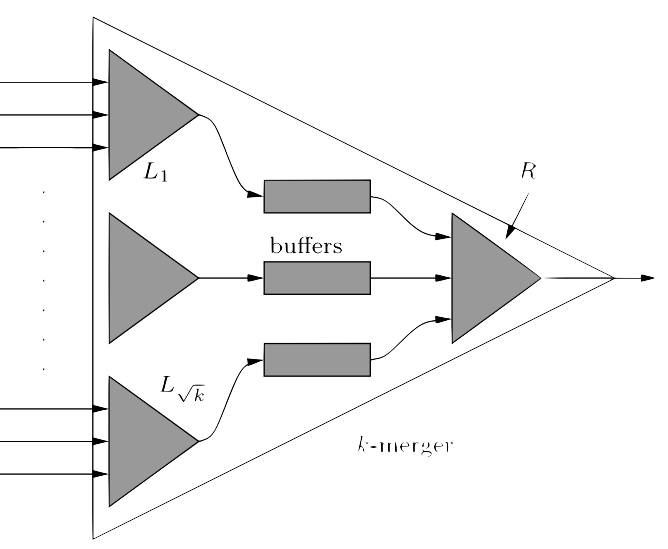
\includegraphics[width=0.85\textwidth]{image3.png}
                \caption{Recursive nature of Funnelsort\ [\cite{frigo}]}
            \end{figure}
        \end{column}
    \end{columns}
\end{frame}

\begin{frame}{Funnelsort: Single $K$-Funnel Instance}

    % A single instance of a \textcolor{MidnightBlue}{$K$-funnel}

    % \vspace{-5pt}
    \begin{columns}[T]

        \begin{column}{0.55\textwidth}
            \begin{itemize}\itemsep0.1em
                \item $K$ input buffers, $1$ output buffer
                \item one \textcolor{MidnightBlue}{$\sqrt{K}$-funnel} at the top
                \item $\sqrt{K}$\ \# of \textcolor{MidnightBlue}{$\sqrt{K}$-funnels} at the bottom
                \item linked by $\sqrt{K}$\ \# of \textcolor{BurntOrange}{middle buffers}
                % \begin{itemize}
                %     \item each buffer size is $K^{3/2}$ 
                %     \item $\sqrt{K} \cdot K^{3/2} = K^2$ total space for all buffers in this $K$-funnel
                % \end{itemize}
                % \\ $\rightarrow$ each buffer size is $K^{3/2}$ 
                % \\ $\implies \sqrt{K} \cdot K^{3/2} = K^2$ total space for all buffers in this $K$-funnel
            \end{itemize}
            % \vspace{0.5cm}
            \textbf{Lazy Merging (The Magic):}
            \begin{itemize}\itemsep0.1em
                \item bottom funnels do not process all \textcolor{ForestGreen}{$K^{5/2}$ data} at once
                \item they run just enough to fill a $K^{3/2}$ \textcolor{BurntOrange}{middle buffer}, then \textcolor{RoyalPurple}{pause}
                \item \texttt{fill()} called on output buffer; and if any of its input buffers are empty, \texttt{fill()} is called on the empty buffer
                % \\sorted chunks only "float up" when the top funnel empties a buffer and demands more data
            \end{itemize}
            
            % $\implies$ each $\sqrt{K}$-funnel at the bottom needs to run $K$ times to process all $\sqrt{K} \cdot K^2 = K^{5/2}$ input data $\implies$ each run it will fill up its $K^{3/2}$ size output buffer, floating up the a chunk of min values
        \end{column}
        \begin{column}{0.45\textwidth}
            \vspace{-15pt}
            \begin{figure}
                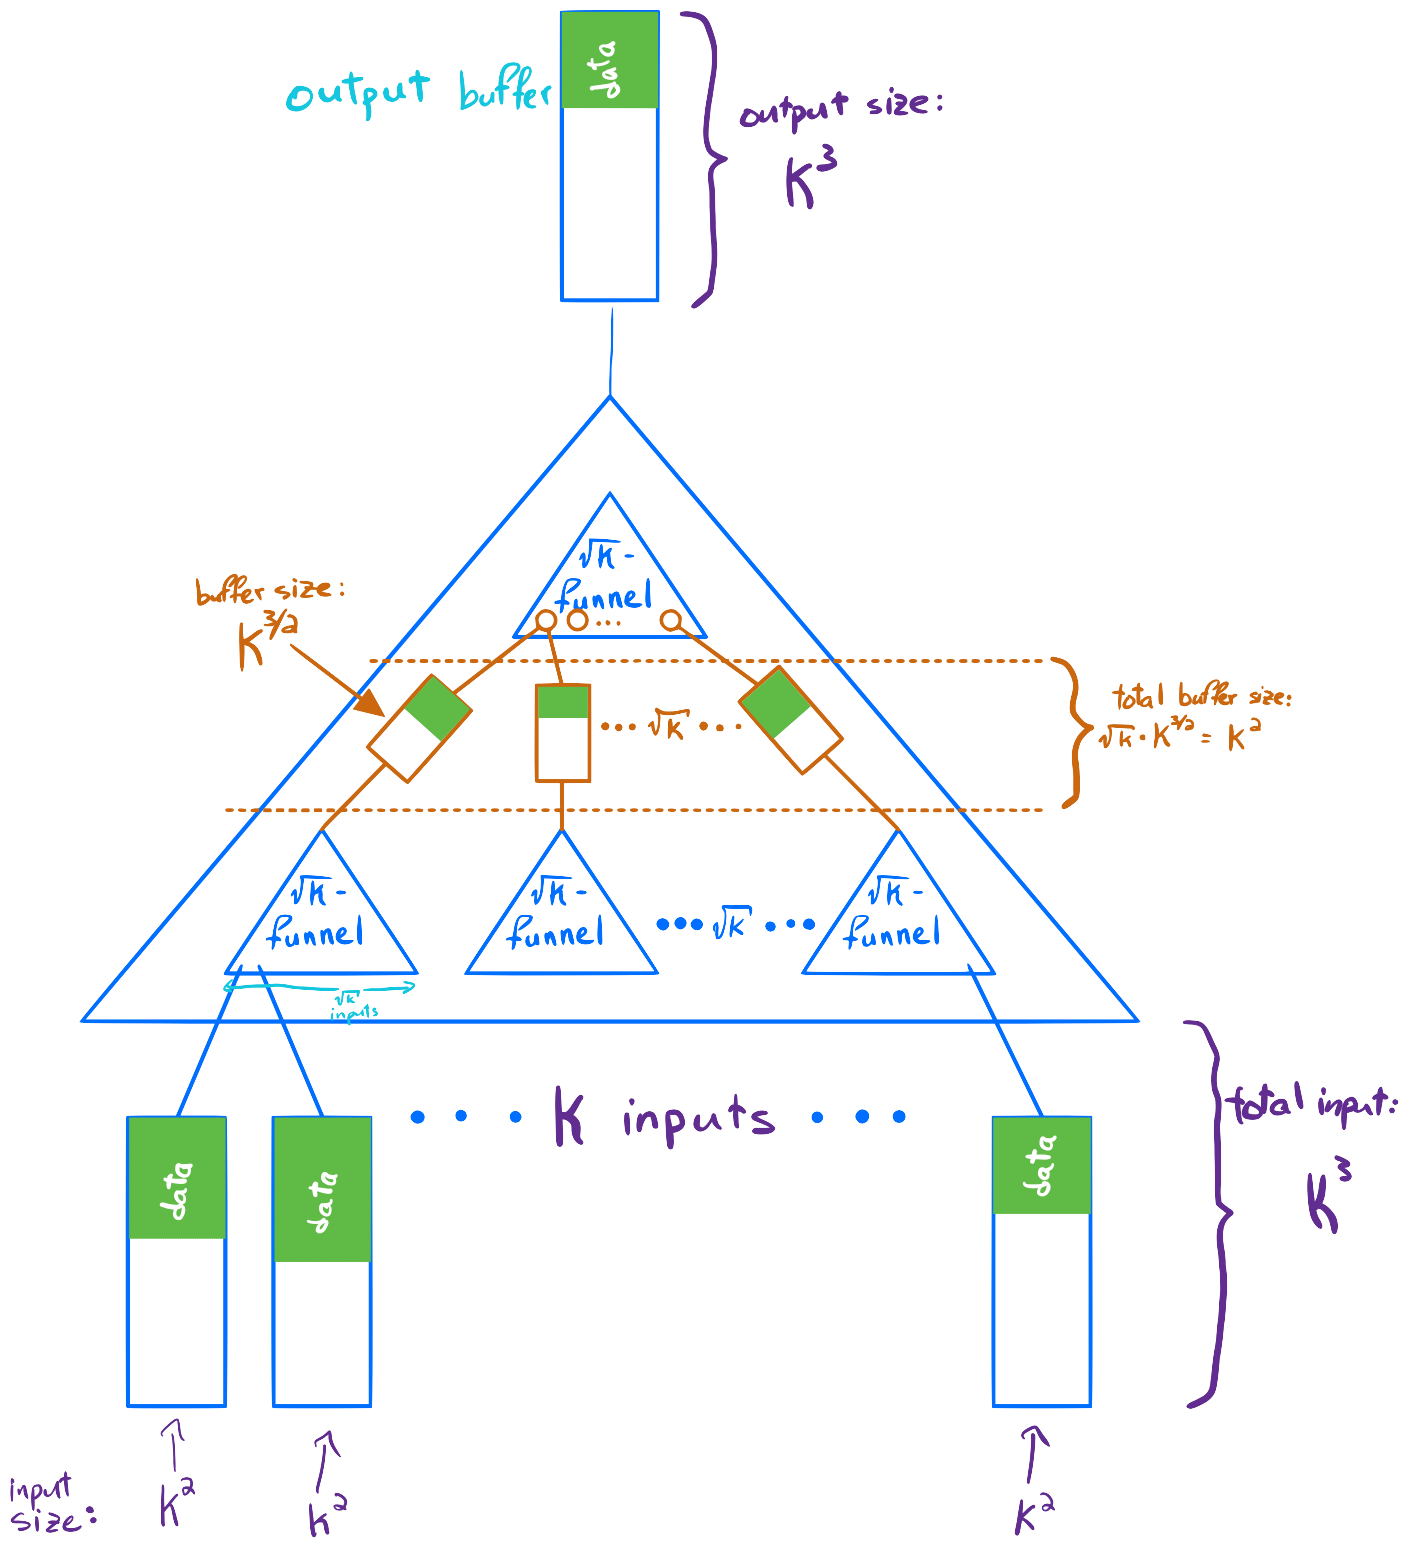
\includegraphics[width=\textwidth]{Page1.png}
            \end{figure}
            
        \end{column}
        
    \end{columns}

\end{frame}

\begin{frame}{Funnelsort: Base Case}

    \begin{columns}[T]

        \begin{column}{0.55\textwidth}
            $K=2 \implies$ \textcolor{MidnightBlue}{$2$-funnel} 
            
            \medskip

            $\implies$ A simple 2-way merge!

            \bigskip
            \begin{itemize}
                \item $2$ input buffers, $1$ output buffer
                \item no nested \textcolor{MidnightBlue}{funnels}
                \item no \textcolor{BurntOrange}{middle buffers}
                \item it simply:
                \begin{itemize}
                    \item fills the output buffer
                    \item then waits to be called again
                    \item repeat
                \end{itemize}
                % \begin{itemize}
                %     \item each buffer size is $K^{3/2}$ 
                %     \item $\sqrt{K} \cdot K^{3/2} = K^2$ total space for all buffers in this $K$-funnel
                % \end{itemize}
                % \\ $\rightarrow$ each buffer size is $K^{3/2}$ 
                % \\ $\implies \sqrt{K} \cdot K^{3/2} = K^2$ total space for all buffers in this $K$-funnel
            \end{itemize}
        \end{column}
        \begin{column}{0.45\textwidth}
            \vspace{-15pt}
            \begin{figure}
                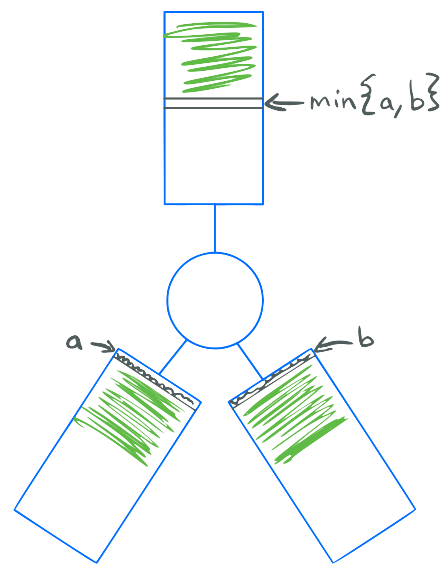
\includegraphics[height=0.9\textheight]{Page2.png}
            \end{figure}
        \end{column}
    \end{columns}
\end{frame}

 

\begin{frame}[allowframebreaks]{References}
    \printbibliography%
\end{frame}

\end{document}